\documentclass[isoft]{ufgtexposter}

\usepackage{lipsum}
\usepackage{natbib}
\usepackage{booktabs}
\usepackage{subfig} 
\usepackage{amsmath} 
\usepackage{textcomp} 
\usepackage{url}  
\usepackage[hidelinks]{hyperref}
\usepackage[utf8]{inputenc}
\usepackage[english]{babel}
\usepackage{graphicx}
%%%%%%%%%%%%%%%%%%%%%%%%%%%%%%%%%%%%%%%%%
%%               Configs               %%
%%%%%%%%%%%%%%%%%%%%%%%%%%%%%%%%%%%%%%%%%

% Choose one of the section color {ufglhblue | ufgdkblue | dkblue | black | gold}
\setsectioncolor{dkblue} 

% Define width of the rule or hide it by setting 0pt or commenting the command 
\setcolumnseprule{3pt}

% Inform the paths to the logo files or leave empty one or both parameters. 
% There are three options [ T | M | B ] to positioning them.

\setlogos[T]{}{images/logos}

% Choose one of the background options {1 | 2 | 3}. 
% Actually, one can select any graphic file in backgrounds directory. 
\setbackground{3}

% Resize the title to keep it in two lines // {font size}{line height}
\settitlesize{64pt}{68pt}

% Resize the font of the content. Default {32pt}{38pt} // {font size}{line height}
\setcontentfontesize{33pt}{34pt}

% Resize the font of the emails. Default {26pt}{32pt} // {font size}{line height}
\setemailfontesize{42pt}{40pt}

% General info
\title{\uppercase{Direct Detection of Exoplanets using Tunable Kernel-Nulling}}

\author{Vincent Foriel, Frantz Martinache, David Mary} 

\department{Univesité Côte d'Azur, Observatoire de la Côte d'Azur Nice, CNRS, Laboratoire Lagrange, France}

\email{ \text{vincent.foriel@oca.eu, frantz.martinache@oca.eu, david.mary@oca.eu} }

\class{}

\posteryear{2024}

\copyrightholder{SPIE - Yokohama, Japan}

%%%%%%%%%%%%%%%%%%%%%%%%%%%%%%%%%%%%%%%%%
%%           End configs               %%
%%%%%%%%%%%%%%%%%%%%%%%%%%%%%%%%%%%%%%%%%

\pagestyle{fancy}

\begin{document}
    \begin{poster}
    %%%%%%%%%%%%%%%%%%%%%%%%%%%%%%%%%%%%%%%%%
    %%             Begin poster            %%
    %%%%%%%%%%%%%%%%%%%%%%%%%%%%%%%%%%%%%%%%%
    
    \section{Abstract}
        
        This thesis proposes an innovative approach, tunable Kernel-Nulling, for high-contrast imaging of exoplanets. Using integrated optics technology with electronically controlled phase shifters, the method asymmetrically modifies the nuller's response, allowing the discrimination of astrophysical signals from diffraction-induced speckles. The device's performance optimization involves machine learning techniques, initially in a controlled setting and later in realistic observing conditions. This approach promises to significantly enhance interferometric high-contrast imaging, providing a powerful solution for achieving deep and robust observations.

        \begin{figure}
            \centering
            \captionsetup{type=figure}
            %mude o scale até sua imagem ficar do tamanho certo o scale pode ter valores menores que 
            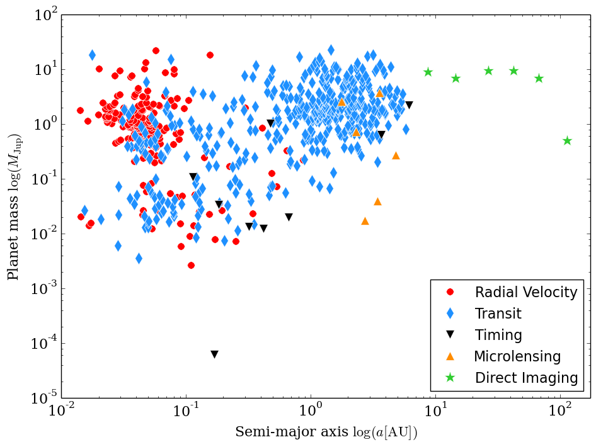
\includegraphics[scale=1.5]{images/detection_technics.png}
            \caption{MeDetections per method. By Paul Anthony Wilson - Exoplanet detection techniques}
            \label{fig:detection_methods}
        \end{figure}

        
    \section{Context}%
        
        \subsection{Nulling interferometry}

            \begin{figure}
                \centering
                \captionsetup{type=figure}
                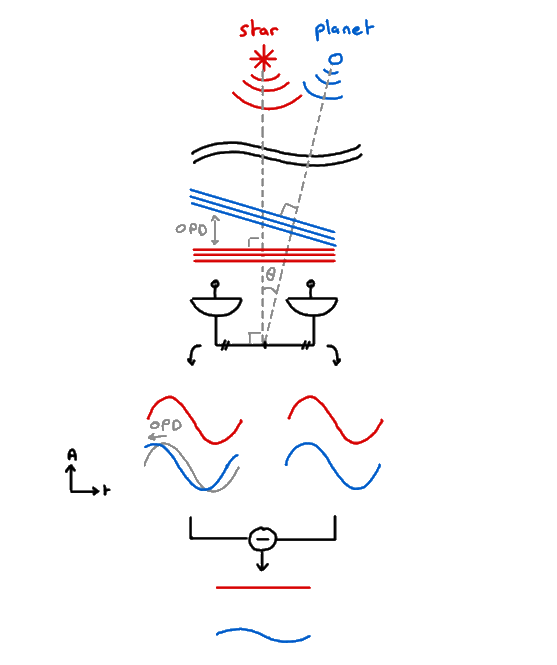
\includegraphics[scale=1.5]{images/nuller_scheme.png}
                \caption{Illustration of the Nulling principle.}
                \label{fig:nulling_principle}
            \end{figure}
        
            By synchronizing the phase of the star light collected by two (or more!) telescopes, it is possible to cancel the star's light. As the star companion is not on the line of sight, it's phase will not be perfectly synchronized and will not be canceled. This is the principle of nulling interferometry.
    
        
        
        \subsection{Our architecture}

        
            \lipsum[54]

            \begin{figure}
                \centering
                \captionsetup{type=figure}
                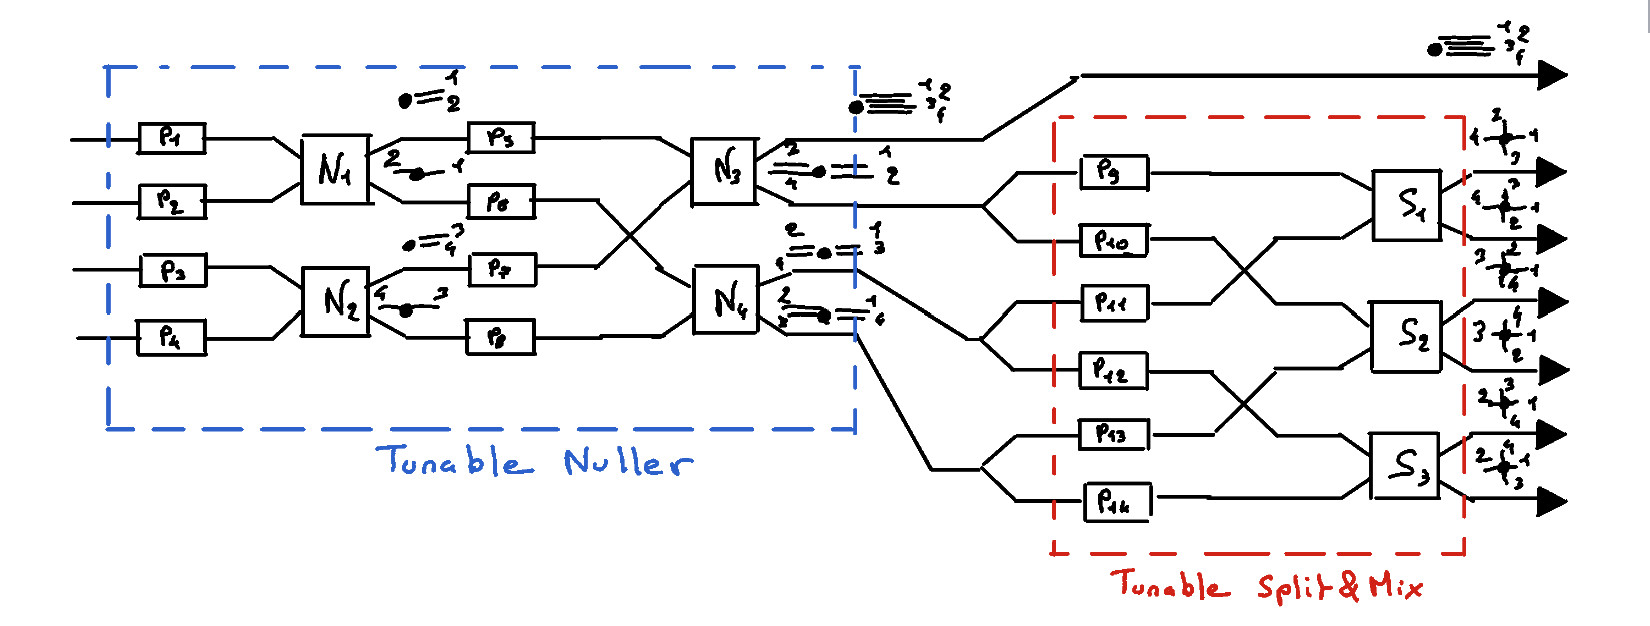
\includegraphics[scale=1.75]{images/architecture_scheme.png}
                \caption{Scheme of our architecture.}
                \label{fig:architecture_scheme}
            \end{figure}

            \begin{figure}
                \centering
                \captionsetup{type=figure}
                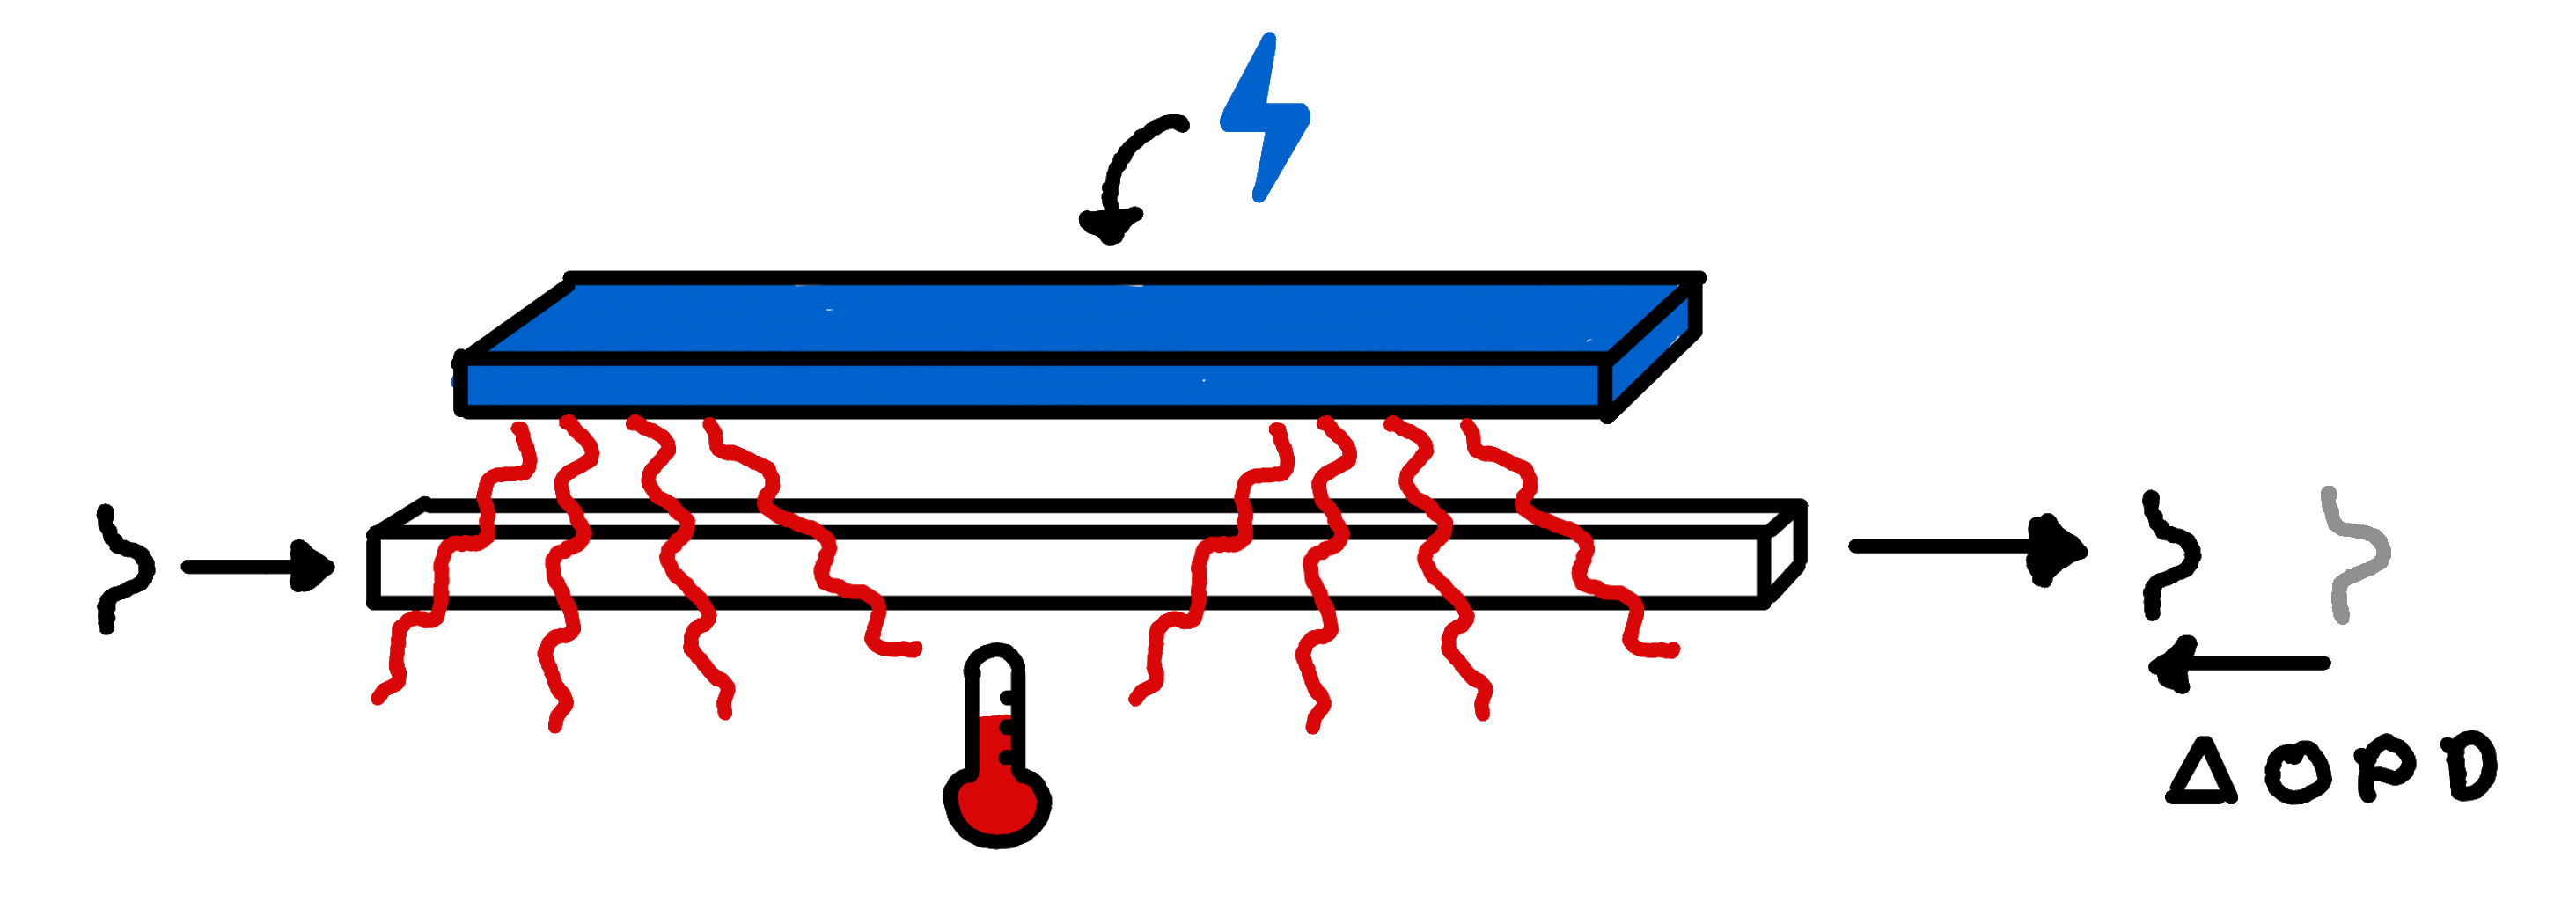
\includegraphics[scale=0.25]{images/thermo-optic_phase_shifter.png}
                \caption{Thermo-optic phase shifter.}
                \label{fig:thermo-optic_phase_shifter}
            \end{figure}

            
            \citep{defects2j}.
    
        \section{Results \& discussion}%
                
            \lipsum[4]    
    
            \vspace{0.5cm}
            %Aaqui começa a tabela
            \begin{table}
                \centering
                \captionsetup{type=table}
                \caption{\textit{Corpus} utilizados no estudo}
                \label{Corpus}
                \renewcommand{\arraystretch}{1.2}
                \resizebox{0.47\textwidth}{!}{%
                \begin{tabular}{lcccclcl}
                    \hline
                    &\textbf{Corpus}    &  \textbf{Caracteres únicos} &    &  \textbf{Total de linhas}  &  & \textbf{Total de caracteres} &  \\ \hline
                    &SBSEThesis         & 88  &    &    2.311     &        & 771.179 &  \\ 
                    &Bible              & 63  &    &    32.359   &        & 3.924.374 &  \\
                    &JavaCode           & 69  &    &    436.565  &        & 12.053.424 &  \\ \hline
                \end{tabular}
            }
            \end{table}
            \vspace{0.5cm}
    
            \cite{chollet2015keras}     
    
        \section{Acknowledgements}
    
            \lipsum[57]
    
        \bibliographystyle{abbrv}
        \bibliography{refs}
    
    %%%%%%%%%%%%%%%%%%%%%%%%%%%%%%%%%%%%%%%%%
    %%               End poster            %%
    %%%%%%%%%%%%%%%%%%%%%%%%%%%%%%%%%%%%%%%%%
    
    \end{poster}

\end{document}

 
